\subsection{Results}\label{sec:ghca_results}
The eventual periodicity of any input is clear from the finite state space.
The only way to achieve a periodicity $< 2$ is if all cells are ready/in state 0 because that is the only state in which a cell does not change its value.
This means that every initial configuration that does not die out becomes periodic with period $\geq 2$.
As the lecture already postulated\cite[Lecture~9, slide~24]{Lecture}, the period in our experimentation depends on the number of states and excited states.
When $N\geq5$ and $e\geq2$ the period is exactly equal to the number of states.
We did not prove this in a complete way, we only encountered no counter-example.
For $e=1$ I found periods $>N$.
An example of this is the period 8 GIF uploaded as \texttt{431\_442\_453.gif} which is the periodic behaviour originating from the configuration shown
\begin{figure}[h]
	\centering
	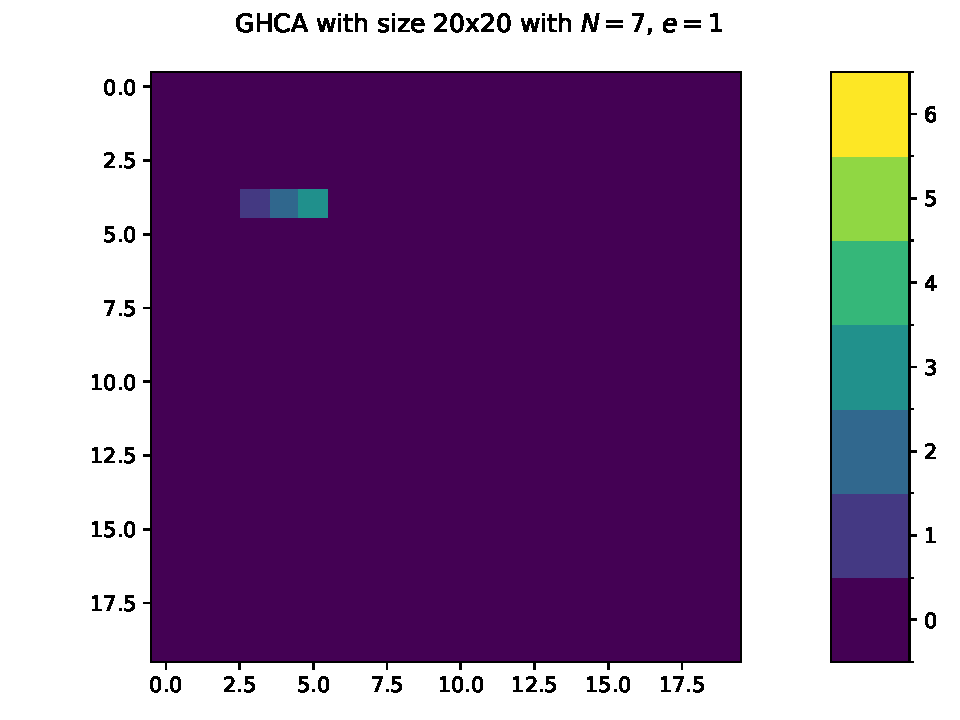
\includegraphics[width=0.7\textwidth]{figs/conf_start_431442453}
	\caption{Simple Starting Configuration for Later Periodic Behaviour}
	\label{fig:startconf}
\end{figure}
in figure \ref{fig:startconf}.
This configuration is also a good way to elucidate the difference between the transient and periodic behaviour.
While the initial configuration is very simple with only three cells being non-zero, the periodic configuration looks a lot more chaotic with different wavefronts.
\begin{figure}[h]
	\centering
	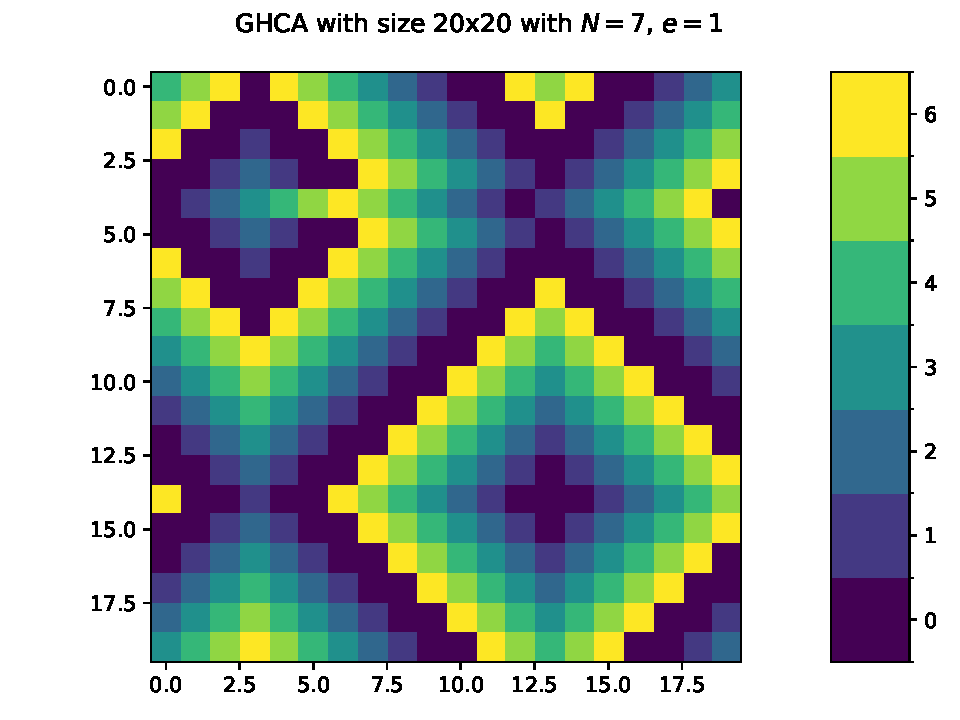
\includegraphics[width=0.7\textwidth]{figs/conf_periodic_431442453}
	\caption{Member of Periodic Orbit Emerged from Simple Configuration}
	\label{fig:periodicconf}
\end{figure}
One member of the periodic orbit is shown in figure \ref{fig:periodicconf}.
The input configuration is supplied with the report as \texttt{periodic\_N7\_e1\_size20.in} in the machine- and human-readable tuple format specifying coordinates and corresponding values.
The values in the filename refer to the corresponding important simulation parameters number of states $N=7$, number of excited states $e=1$ and edge length $\mathrm{size}=20$.